\documentclass[utf8x, 12pt]{G7-32}
\sloppy

% 1. Настройки стиля ГОСТ 7-32
% Для начала определяем, хотим мы или нет, чтобы рисунки и таблицы нумеровались в пределах раздела, или нам нужна сквозная нумерация.
% А не забыл ли автор букву 't' ?
\EqInChapter % формулы будут нумероваться в пределах раздела
\TableInChapter % таблицы будут нумероваться в пределах раздела
\PicInChapter % рисунки будут нумероваться в пределах раздела

% 2. Добавляем гипертекстовое оглавление в PDF
\usepackage[
bookmarks=true, colorlinks=true, unicode=true,
urlcolor=black,linkcolor=black, anchorcolor=black,
citecolor=black, menucolor=black, filecolor=black,
]{hyperref}

% 3. Изменение начертания шрифта --- после чего выглядит таймсоподобно.
% apt-get install scalable-cyrfonts-tex

\IfFileExists{cyrtimes.sty}
    {
        \usepackage{cyrtimespatched}
    }
    {
        % А если Times нету, то будет CM...
    }


% 4. Прочие полезные пакеты.
\usepackage{underscore} % Ура! Теперь можно писать подчёркивание.
                        % И нельзя использовать подчёркивание в файлах.
                        % Выбирай, но осторожно.

\usepackage{graphicx}   % Пакет для включения рисунков

 % 5. Любимые команды
\newcommand{\Code}[1]{\textbf{#1}}

% 6. Поля
% С такими оно полями оно работает по-умолчанию:
% \RequirePackage[left=20mm,right=10mm,top=20mm,bottom=20mm,headsep=0pt]{geometry}
% Если вас тошнит от поля в 10мм --- увеличивайте до 20-ти, ну и про переплёт не забывайте:
\geometry{right=20mm}
\geometry{left=30mm}


% 7. Tikz
\usepackage{tikz}
\usetikzlibrary{arrows,positioning,shadows}

% 8 Листинги

\usepackage{listings}

% Значения по умолчанию
\lstset{
  basicstyle= \footnotesize,
  breakatwhitespace=true,% разрыв строк только на whitespacce
  breaklines=true,       % переносить длинные строки
%   captionpos=b,          % подписи снизу -- вроде не надо
  inputencoding=koi8-r,
  numbers=left,          % нумерация слева
  numberstyle=\footnotesize,
  showspaces=false,      % показывать пробелы подчеркиваниями -- идиотизм 70-х годов
  showstringspaces=false,
  showtabs=false,        % и табы тоже
  stepnumber=1,
  tabsize=4,              % кому нужны табы по 8 символов?
  frame=single
}

% Стиль для псевдокода: строчки обычно короткие, поэтому размер шрифта побольше
\lstdefinestyle{pseudocode}{
  basicstyle=\small,
  keywordstyle=\color{black}\bfseries\underbar,
  language=Pseudocode,
  numberstyle=\footnotesize,
  commentstyle=\footnotesize\it
}

% Стиль для обычного кода: маленький шрифт
\lstdefinestyle{realcode}{
  basicstyle=\scriptsize,
  numberstyle=\footnotesize
}

% Стиль для коротких кусков обычного кода: средний шрифт
\lstdefinestyle{simplecode}{
  basicstyle=\footnotesize,
  numberstyle=\footnotesize
}

% Стиль для BNF
\lstdefinestyle{grammar}{
  basicstyle=\footnotesize,
  numberstyle=\footnotesize,
  stringstyle=\bfseries\ttfamily,
  language=BNF
}

% Определим свой язык для написания псевдокодов на основе Python
\lstdefinelanguage[]{Pseudocode}[]{Python}{
  morekeywords={each,empty,wait,do},% ключевые слова добавлять сюда
  morecomment=[s]{\{}{\}},% комменты {а-ля Pascal} смотрятся нагляднее
  literate=% а сюда добавлять операторы, которые хотите отображать как мат. символы
    {->}{\ensuremath{$\rightarrow$}~}2%
    {<-}{\ensuremath{$\leftarrow$}~}2%
    {:=}{\ensuremath{$\leftarrow$}~}2%
    {<--}{\ensuremath{$\Longleftarrow$}~}2%
}[keywords,comments]

% Свой язык для задания грамматик в BNF
\lstdefinelanguage[]{BNF}[]{}{
  morekeywords={},
  morecomment=[s]{@}{@},
  morestring=[b]",%
  literate=%
    {->}{\ensuremath{$\rightarrow$}~}2%
    {*}{\ensuremath{$^*$}~}2%
    {+}{\ensuremath{$^+$}~}2%
    {|}{\ensuremath{$|$}~}2%
}[keywords,comments,strings]

% Подписи к листингам на русском языке.
\renewcommand*\thelstnumber{\oldstylenums{\the\value{lstnumber}}}
\renewcommand\lstlistingname{\cyr\CYRL\cyri\cyrs\cyrt\cyri\cyrn\cyrg}
\renewcommand\lstlistlistingname{\cyr\CYRL\cyri\cyrs\cyrt\cyri\cyrn\cyrg\cyri}

% Произвольная нумерация списков.
\usepackage{enumerate}


\begin{document}

\frontmatter

\Defines
\begin{description}
        \item[Распределённая система обработки информации] система взаимодействующих
        независимых автоматизированных информационных систем, каждая из которых 
        принадлежит и администрируется различными организациями (лицами), которые 
        преследуют свои собственные цели.
        \item[Участник РСОИ] независимая автоматизированная информационная система,
        входящая в состав распределенной системы обработки информации.  
        \item[Сообщение] минимально передаваемая единица полезной информации.
        \item[Заявка] единица обслуживания.
        \item[Протокол  обмена] это пятёрка:
                \begin{enumerate}
                        \item назначение протокола (предоставляемые им возможности);
                        \item используемый нижестоящий протокол или протоколы;
                        \item алфавит;
                        \item словарь сообщений и синтаксис сообщений;
                        \item возможная последовательность сообщений и их семантика.
                \end{enumerate}
        \item[Жизненный цикл заявки] конечное множество возможных состояний заявки.
        \item[Релевантность] способность информации соответствовать постребностям.
\end{description}

\Abbreviations
\begin{description}
	\item[РСОИ] Распределённая система обработки информации
	\item[АИС] Автоматизированная информационная система
	\item[БД] База данных
	\item[ЛПО] Логика предметной области
	\item[ИП] Интерфейс пользователя
	\item[ПОЗ] Подсистема обработки заявок
	\item[ПФС] Подсистема фильтрации сообщений
	\item[ПОС] Подсистема обмена сообщениями
	\item[ПС] Подсистема статистики
	\item[ПФЗ] Подсистема фильтрации заявок
	\item[ПО] Программное обеспечение
	\item[ПП] Программный продукт
\end{description}

\mainmatter

\chapter{Введение}
Данное техническое задание составлено для проектирования ПО "Подсистема 
фильтрации нежелательных заявок участника РСОИ". Техническое задание выполнено на 
основе ГОСТ 19.201-78. "ЕСПД. Техническое задание. Требования к содержанию и 
оформлению".

\section{Краткое описание предметной области}
Типичная структура РСОИ представлена на рис. ~\ref{fig:rsoi}. АИС, входящие в 
состав РСОИ  являются независимыми и не могут ни получить полностью достоверную 
информацию о состоянии других систем на заданный момент времени, ни польностью 
контролировать её поведение. Каждая из АИС имеет свою логику работы (с точки 
зрения других участников эта логика полностью не просматривается) и свою БД 
или несколько БД, в которых хранит состояние своей модели предметной области. 
Прямой доступ не уровне SQL к этим БД другим участникам не даётся, даже на чтения 
с ограниченными правами. В силу этого системы могут могут выдавать упрощённую или 
искажённую информацию другим участникам РСОИ. В общем случае для создания 
РСОИ всем организациям, владеющим непосредственно взаимодействующими 
учатсниками РСОИ необходимо заключить друг сдругои договор.
\begin{figure}
        \centering
        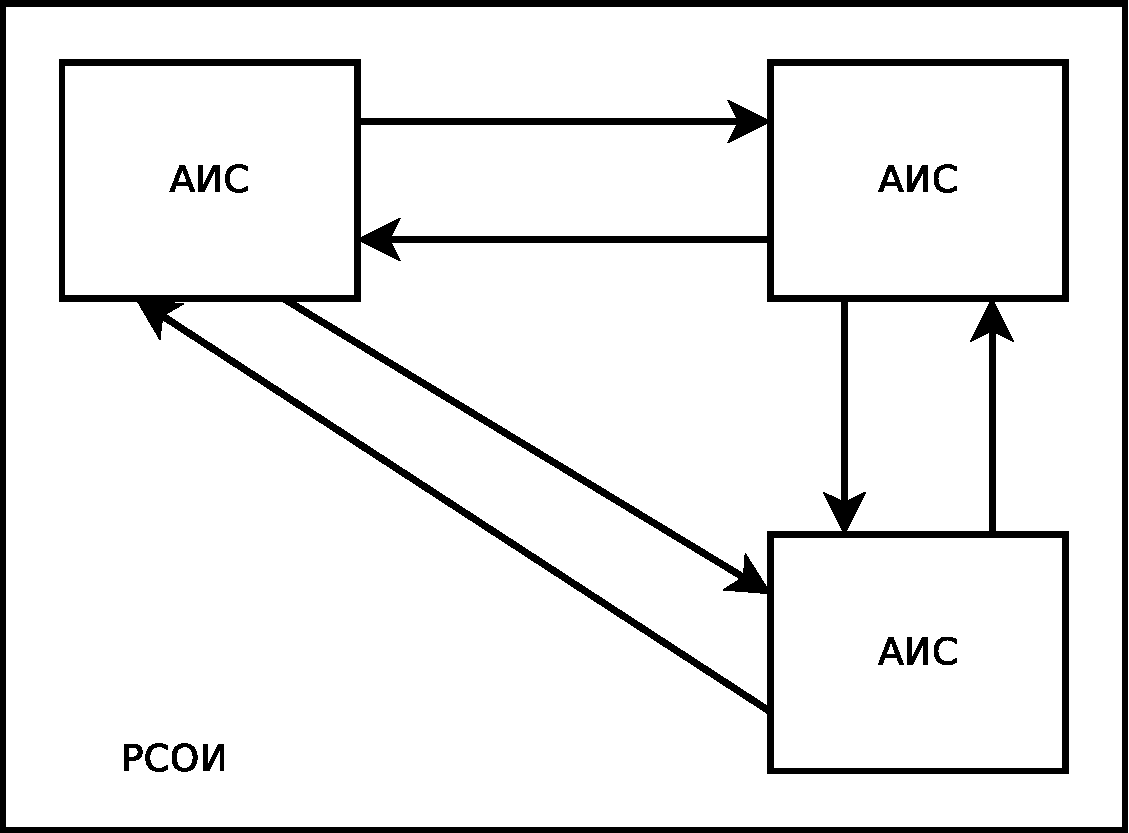
\includegraphics[width=0.5\textwidth]{inc/dia/rpz-rsoi}
        \caption{Структура РСОИ, состоящей из 3 независимых АИС}
        \label{fig:rsoi}
\end{figure}

Структура участника РСОИ в общем случае показана на рис. ~\ref{fig:participant}. 
\begin{figure}
        \centering
        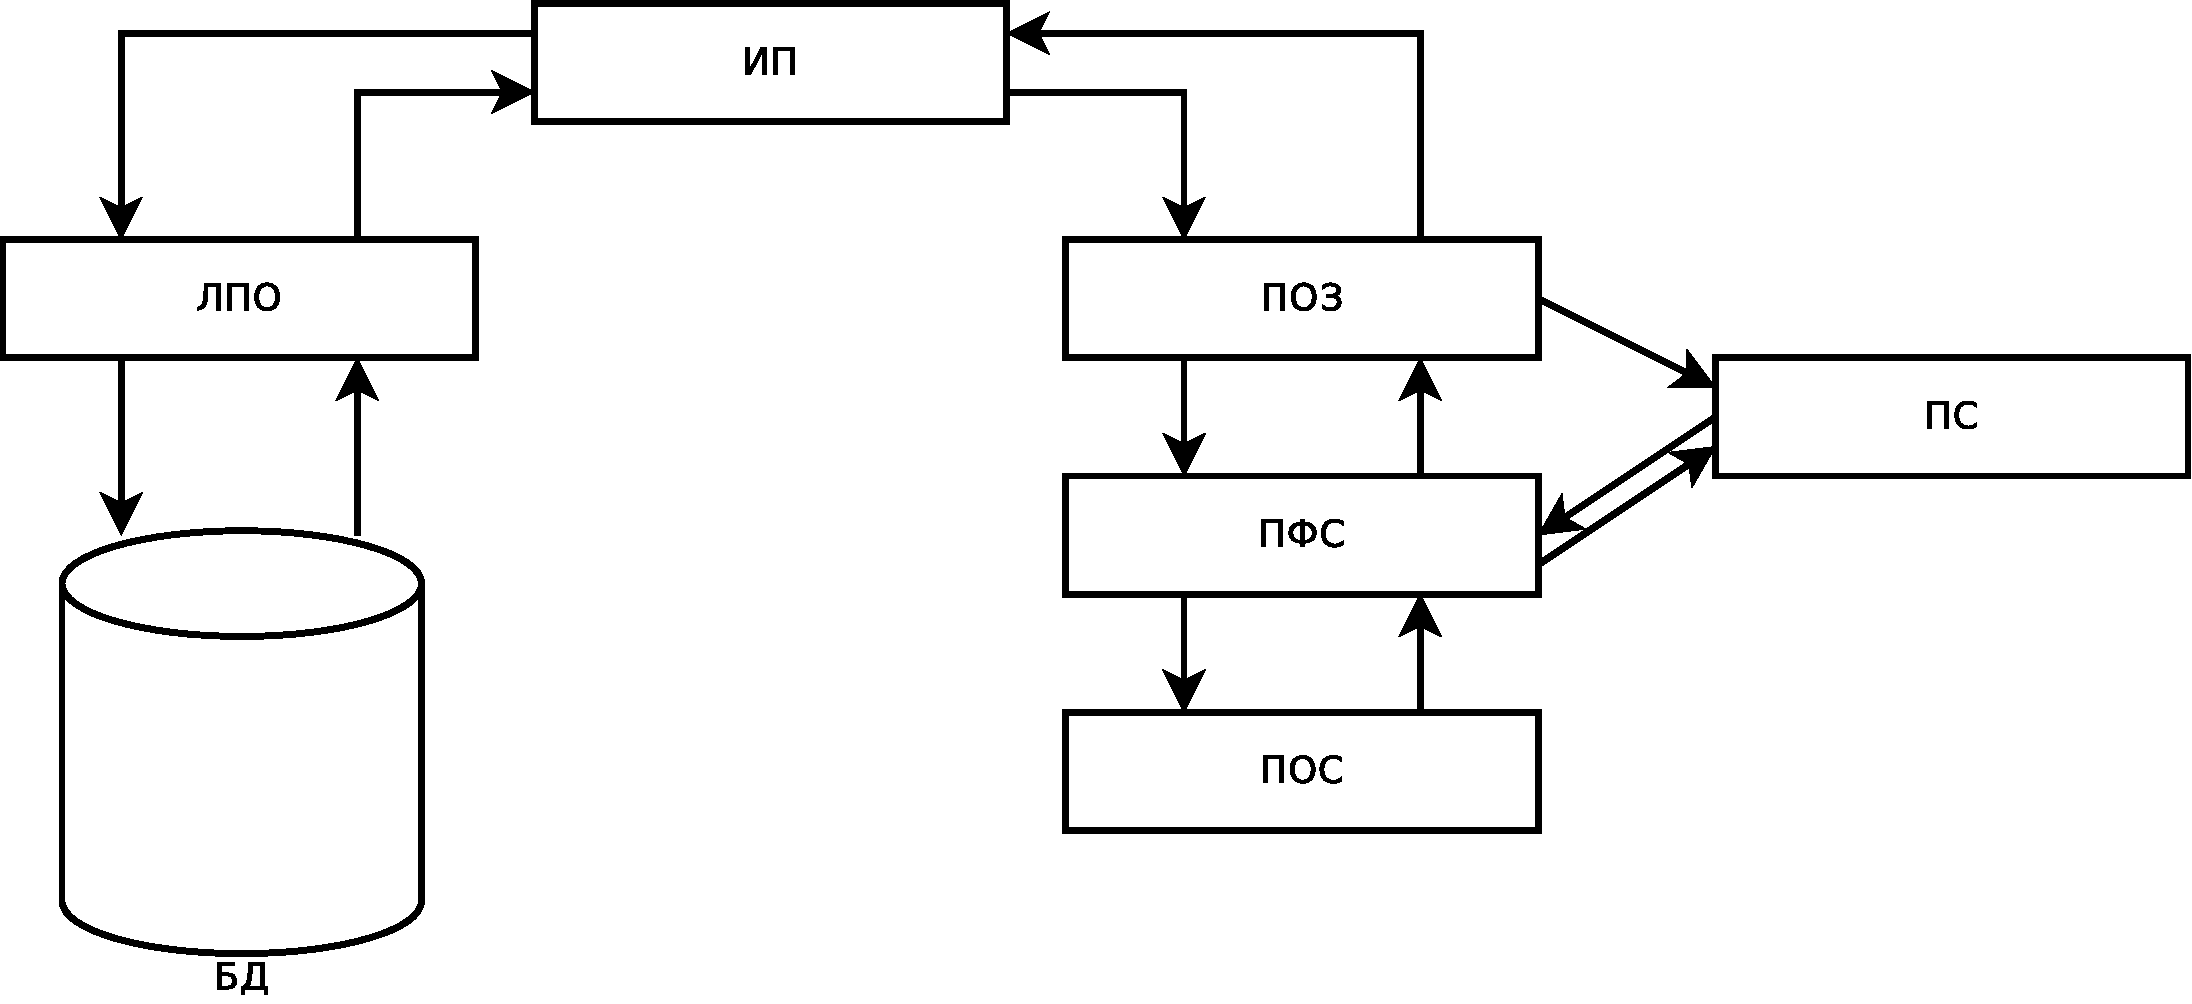
\includegraphics[width=0.7\textwidth]{inc/dia/rpz-participant}
        \caption{Структура участника РСОИ}
        \label{fig:participant}
\end{figure}
ПОС занимается вопросами преобразования полученных от ПОЗ сообщений в форму.
понятную другим системам, и принимаемых от других систем сообщений в форму,
понятную непосредственно самой системе. ПФС фильтрует сообщения во внутреннем 
представлении, чтобы не загружать систему работой, которая выглядит 
неправдоподобной. Входящая в её состав ПФЗ выносит "вердикт" по заявкам, 
полученным от других систем, исходя из которого протокол обмена предпринимает те или 
иные дальнейшие шаги. Решение принимается на основе:
\begin{enumerate}
        \item текущего состояния модели предметной области;
        \item истории взаимоотнощений с партнёрами;
        \item параметров заявки (например, количестве запрашиваемых ресурсов);
        \item правил принятия решений.
\end{enumerate}
ПОЗ является ключевой с точки зрения участия в распределенной системе. Она 
реализует часть высокоуровнего простокола участника РСОИ. связанную с жизненным 
циклом выполнения заявки.

\section{Существующие аналоги}
В настоящее время нет аналогичных ПП, позволяющих выполнить анализ релевантности
и соответственно фильтрацию заявок на основе недельно-сезонных колебаний без 
привязки к конкретной предметной области.

\section{Описание подсистемы фильтрации заявок}
	Главное назначение ПО "Подсистема фильтрации нежелательных заявок участника 
РСОИ" - определение релевантности поступающих в систему заявок. Алгоритм работы 
подсистемы показан на рис. ~\ref{fig:algorithm}.
\begin{figure}
        \centering
        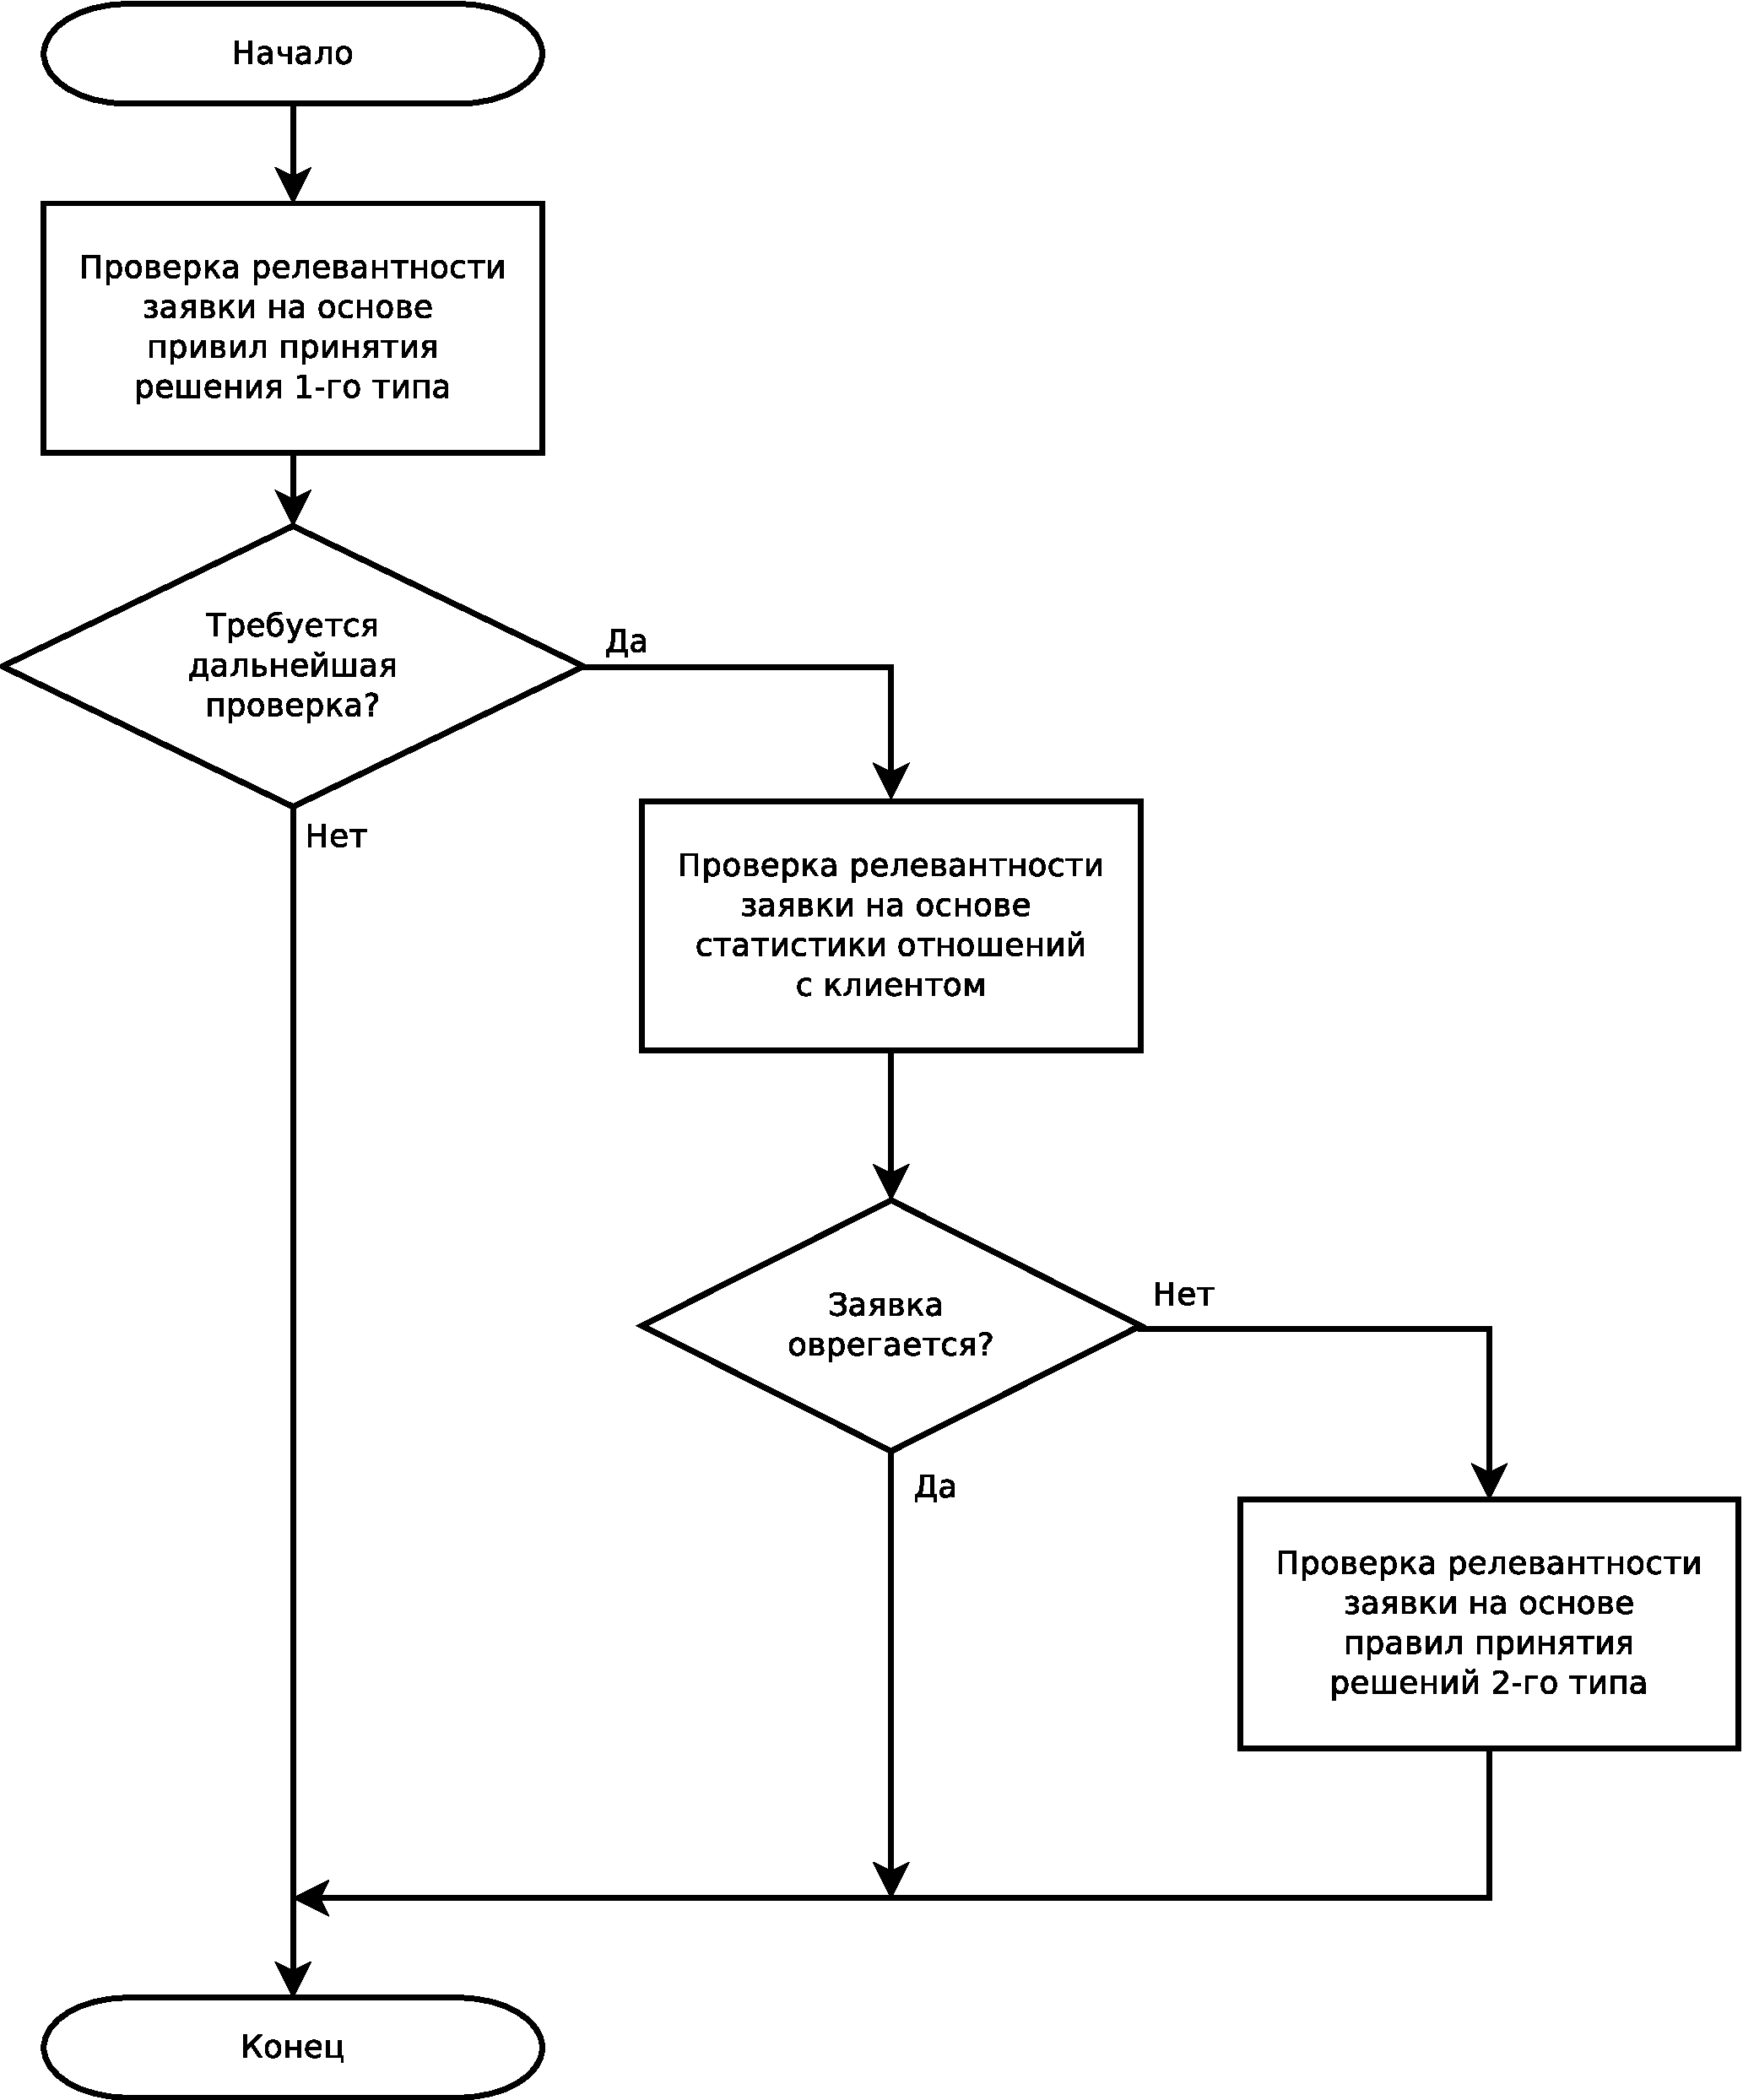
\includegraphics[width=0.7\textwidth]{inc/dia/rpz-algorithm}
        \caption{Алгоритм определения релевантности заявки}
        \label{fig:algorithm}
\end{figure}
Для определения релевантности заявки на основе статистики отношений с клиентом
подсистеме необходимо пройти предварительное обучение с использованием данных,
предоставляемых ей ПС. Правила принятия решений задают дополнительные 
ограничения, накладываемые на поступающие заявки, исходя из здравого смысла и 
бизнес-логики работы системы. Как видно из рисунка правила бывают двух типов.
Выполнение правил 1-го типа проверяется до проверки релевантности системы на
основе статистики отношений с клиентом (например, для данного клиента  
пропускать все поступающие заявки без анализа статистики отношений с ним и т.п.). 
А выполнение правил 2-го типа проводится после него в случае, если заявка была
признана релевантной, исходя из статистики отношений с клиентом (например, заявка на 
количество ресурса, большее половины имеющихся на данный момент в системе, 
признается нерелевантной).

\nobreakingbeforechapters
\chapter{Основания для разработки}

Разработка ведётся в рамках выполнения лабораторных работ по курсу "Методология
программной инженерии" на основе утверждённого учебного плана и в рамках курсового
проектирования по курсу "Рапределённые системы обработки информации".

\chapter{Назначение разрабоки}

ПО "Подсистема фильтрации нежелательных заявок участника РСОИ"  предназначено
для определения релевантности заявок, поступающих в систему от других учестников
РСОИ.

\chapter{Требования к программному изделию}

\section{Требования к подсистеме}

\begin{enumerate}
        \item Разрабатываемое ПО должно обеспечить функционирование подсистемы
        в режиме 24/7/365.
        \item Время восстановления после сбоя должно составлять не более 1 часа.
\end{enumerate}

\section{Требования к функциональным характеристикам}

\begin{enumerate}
        \item Подсистема должна поддерживать возможность переобучения системы без
        прерывания её функционирования более, чем на 3 минуты.
        \item Подсистема должна обеспечить обработку не  менее 100 заявок в минуту.
        \item Количество неправильно классифицированных заявок за сутки должно 
        составлять не более 5\% от общей массы заявок, поступающих в систему за этот 
        период.
\end{enumerate}

\section{Функциональные требования с точки зрения участника РСОИ}

Подсистема фильтрации заявок должна обечпечить выполнение следующих функций:

Входные параметры подсистемы
Выходные параметры подсистемы

\section{Требования к надёжности}

Для повышения надёжности работы подсистемы необходимо:
\begin{enumerate}
        \item производить переобучение подсистемы не реже 1 раза в неделю;
        \item производиться журналирование поступающих заявок и принимаемых 
        подсистемой решений;
        \item срок хранения принятых подсистемой решений должен составлять не менее
        3 недель.
\end{enumerate}

\section{Требования к составу и параметрам технических средств}

Минимальные технические требования:
\begin{enumerate}
        \item 2-х ядерный процессор с тактовой частотой 2ГГц;
        \item ОЗУ 4 ГБ;
        \item сетевая карта Ethernet стандарта 1000BASE-T.
\end{enumerate}

Требования к операционному окружению:
\begin{enumerate}
        \item Операционные системы: Windows XP/7, Ubuntu 11.04.
\end{enumerate}

\section{Требования к информационной и программной совместимости}
Разработка должна вестись с использованием открытого платформенно-независимого ПО.

\section{Требования к документации}

Документация должна включать:
\begin{enumerate}
        \item руководство по развертыванию подсистемы;
        \item руководство по конфигурированию подсистемы;
\end{enumerate}

\backmatter

%\bibliographystyle{gost780u}
%\bibliography{rpz}

\end{document}

%%% Local Variables:
%%% mode: latex
%%% TeX-master: t
%%% End:
